\documentclass[t, 11pt]{beamer}
\pdfmapfile{+sansmathaccent.map}
%%% Работа с русским языком
\usepackage{cmap}				
\usepackage{mathtext} 				
\usepackage[T2A]{fontenc}		
\usepackage[utf8]{inputenc}			
\usepackage[english,russian]{babel}	

\usetheme{Ilmenau}
\usecolortheme{lily} % Цветовая схема



%%% Работа с картинками
\usepackage{graphicx}

\usepackage{csquotes}

\hypersetup{				
	colorlinks=true,       	
	linkcolor=blue,          
	citecolor=black,       
	filecolor=magenta,      
	urlcolor=red           
}


\title{Preprocessing}
%\subtitle{...and it's applications}
\author{Чувакин Сергей}
\date{\today}
\institute{R meetup}

\begin{document}
	\frame[plain]{\titlepage}
	\section{Outline}
	
	\begin{frame}
		\frametitle{\insertsection} 
		\begin{block} {}
			 
			\hyperlink{l1}{\beamerbutton{Vectorization}}
		\end{block}
			\begin{block}{}
		\hyperlink{l1.2}{\beamerbutton{Data cleaning}}
		\end{block}
		\begin{block}{}
			\hyperlink{l2}{\beamerbutton{Tokenization et Normalization}}
		\end{block}
		\begin{block}{}
			\hyperlink{l3}{\beamerbutton{BOW}}
		\end{block}
		\begin{block}{}
			\hyperlink{l4}{\beamerbutton{TF-IDF}}
		\end{block}
			\begin{block}{}
		\hyperlink{l5}{\beamerbutton{N-grams}}
		\end{block}
	\end{frame}
	
	\subsection{Vectorization}
	\begin{frame} \label {l1}
		\frametitle{\insertsection} 
		\frametitle{\insertsubsection} 
		Векторизация - процесс превращения в текста на естесственном языке в вектора. 
		\vspace{1cm}
		\begin{itemize}
			\item \emph{Rule-based} 
			\item Обучение  
		\end{itemize}
	\end{frame}


	\subsection{Pipline} \label{}
	
	\begin{frame}
		\frametitle{\insertsection}
		\frametitle{\insertsubsection}  
	\begin{itemize}

	\item Чистка данных (<<tidy data>>, tags, stop-words)

	\item Нормализация (stemming, lemmatization)

	\item N-grams (?)

	\item Векторизация (simple bow, tf-idf)

	\item Уменьшение размерности (hash trick)
	 \end{itemize}
	\end{frame}

	\subsection{Data cleaning} \label{l1.2}
	
	\begin{frame}
	\frametitle{\insertsection}
	\frametitle{\insertsubsection}  
	\begin{itemize}
		\item Убрать служебные слова
		\item stop-words
	\end{itemize}
\end{frame}


	\subsection{Tokenization}

\begin{frame}\label{l2}
	\frametitle{\insertsection}
	\frametitle{\insertsubsection}
	 \emph{What is text?}
	 
	 \vspace{0.5cm}
	 Токенизация - разделение текста на токены. 
	 \begin{itemize}
	 	\item Буквы 
	 	\item Слова 
	 	\item Фразы
	 	\item Параграфы 
	 	\item etc...
	 	\end{itemize}
 	
\end{frame}

\begin{frame}\label{}
	\frametitle{\insertsection}
	\frametitle{\insertsubsection}
 \begin{enumerate}
 	\item Японский, немецкий, адыгейский, аварский языки. 
 	\item Знаки препинания, апострофы, отрицания.
 \end{enumerate}
\end{frame}


	\subsection{Normalization}

\begin{frame}\label{}
	\frametitle{\insertsection}
	\frametitle{\insertsubsection}
	Стемминг - удаление суфиксов и окончаний у слов. Процесс основан на правилах.
	
	\vspace{1cm}
	Лемматизация - превращение слова в словарную форму. Процесс основанных на словарях.
\end{frame}

	
	\subsection{Stemming}
	
	\begin{frame}\label{}
		\frametitle{\insertsection}
		\frametitle{\insertsubsection}
		Porter, Martin F. 1980.An algorithm for suffix stripping. Program 14 (3): 130-137.  
	
	\vspace{1cm}
	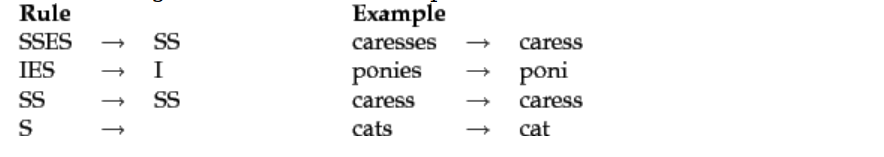
\includegraphics[width=\linewidth]{stem.png}
	\end{frame}
	
	\begin{frame}\label{}
	\frametitle{\insertsection}
	\frametitle{\insertsubsection}
\begin{itemize}
	\item Lovins stemmer
	\item Porter stemmer
	\item Paice stemmer
\end{itemize}
\end{frame}
	
	
	\begin{frame}\label{}
	\frametitle{\insertsection}
	\frametitle{\insertsubsection}
 
	
	%\vspace{1cm}
	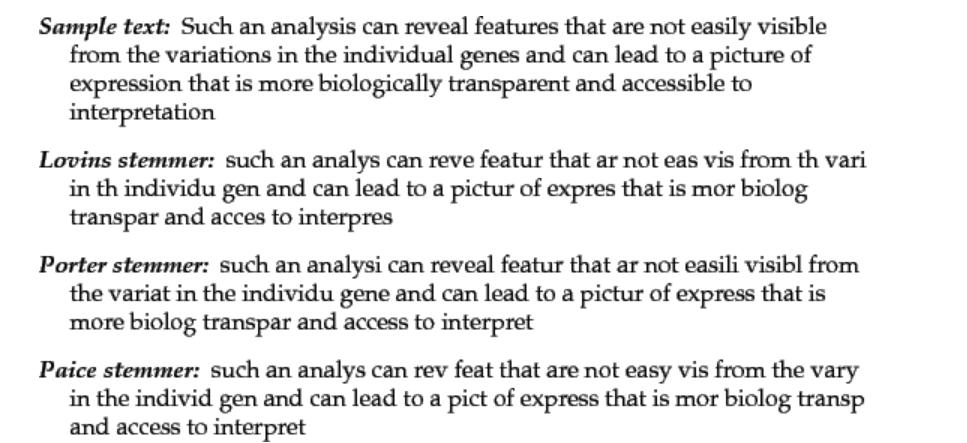
\includegraphics[width=\linewidth]{troi.png}
\end{frame}
\subsection{Stemming vs. Lemmatization}
	\begin{frame}\label{}
	\frametitle{\insertsection}
	\frametitle{\insertsubsection}
	
	
	%\vspace{1cm}
	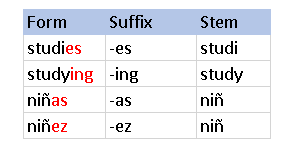
\includegraphics[width=0.4\linewidth]{stem2.png}
	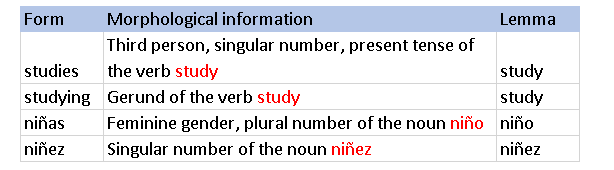
\includegraphics[width=0.7\linewidth]{lem.png}
\end{frame}




		\subsection{BOW}
	\begin{frame}\label{l3}
		\frametitle{\insertsection}
		\frametitle{\insertsubsection}
		Steps: 
		\begin{enumerate}
			\item Make a dictionary.
			\item Create zero vectors.  
			\item Fill with values corresponding the words.
			\item Scoring words
		\end{enumerate}
	\end{frame}

		\subsection{TF-IDF}
		\begin{frame} \label{l4}
			\frametitle{\insertsection}
			\frametitle{\insertsubsection}
	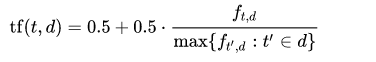
\includegraphics[width=0.5\linewidth]{tf.png}
	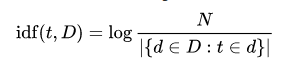
\includegraphics[width=0.5\linewidth]{idf.png}
	%TF термина а = (Количество раз, когда термин а встретился в тексте / количество всех слов в тексте)
%TODO: idf Он считается как логарифм от общего количества документов, делённого на количество документов, в которых встречается термин а.
\end{frame}

		
\begin{frame} \label{}
	\frametitle{\insertsection}
	\frametitle{\insertsubsection}
	
	\begin{enumerate}

\item \textbf{Term Frequency}: is a scoring of the frequency of the word in the current document.
\item \textbf{Inverse Document Frequency}: is a scoring of how rare the word is across documents.

	\end{enumerate}



\end{frame}

			\subsection{N-grams}
	\begin{frame}\label{l5}
		\frametitle{\insertsection}
		\frametitle{\insertsubsection}
		Example: <<It was the best of times>>
		\begin{enumerate}
			\item it was
			\item was the  
			\item the best
			\item best of
			\item of times
		\end{enumerate}
	\end{frame}
	
	
	
			\subsection{Hash trick}
\begin{frame} 
	\frametitle{\insertsection}
	\frametitle{\insertsubsection}
Хэшинг - алгоритм представления строк в виде числа. 
	\begin{enumerate}
		\item есть разные имплементации
		\item можно варьировать длину и размер массива
		\item хорошо подходит для уменьшения размера больших корпусов
		\item замена словарю
	\end{enumerate}
\end{frame}

\end{document}